\documentclass[12pt,letterpaper]{article}
\usepackage[utf8]{inputenc}
\usepackage[spanish]{babel}
\DeclareUnicodeCharacter{03B5}{\ensuremath{\varepsilon}}
\DeclareUnicodeCharacter{2192}{\ensuremath{\rightarrow}}
\usepackage[top=3.4cm,bottom=3cm,left=3cm,right=3.5cm,headheight=48pt,headsep=14pt]{geometry}
\usepackage{graphicx}
\usepackage{amsmath,amssymb}
\usepackage{booktabs}
\usepackage{float}
\usepackage{caption}
\captionsetup[table]{skip=8pt}
\captionsetup[lstlisting]{skip=4pt}
\usepackage{listings}
\usepackage{fancyhdr}
\usepackage{xcolor}
\usepackage{microtype}
\usepackage[hidelinks]{hyperref}

\graphicspath{{../img/}}

\pagestyle{fancy}
\fancyhf{}
\fancyhead[L]{\small\textit{\nouppercase{\rightmark}}}
\fancyhead[R]{\raisebox{-3pt}{
\includegraphics[height=1.45cm]{escudo_usa.png}}\hspace*{-1.2cm}}
\fancyfoot[C]{\thepage}
\renewcommand{\headrulewidth}{0.5pt}
\fancypagestyle{plain}{\fancyhf{}\fancyfoot[C]{\thepage}\renewcommand{\headrulewidth}{0pt}}

\lstset{
  basicstyle=\ttfamily\small,
  columns=fullflexible,
  keepspaces=true,
  showstringspaces=false,
  breaklines=true,
  xleftmargin=2em,
  aboveskip=0.8em,
  belowskip=0.8em,
  captionpos=t,
  extendedchars=true,
  literate={á}{{\'a}}1 {é}{{\'e}}1 {í}{{\'i}}1 {ó}{{\'o}}1 {ú}{{\'u}}1
           {ñ}{{\~n}}1 {Á}{{\'A}}1 {É}{{\'E}}1 {Í}{{\'I}}1 {Ó}{{\'O}}1
           {Ú}{{\'U}}1 {Ñ}{{\~N}}1 {ü}{{\"u}}1 {¿}{{?`}}1 {¡}{{!`}}1
           {ε}{{$\varepsilon$}}1 {→}{{$\rightarrow$}}1
}

\setlength{\parskip}{0.45em}
\setlength{\parindent}{0pt}
\setlength{\emergencystretch}{3em}

\newcommand{\tk}[1]{\texttt{#1}}
\newcommand{\nt}[1]{\textit{#1}}
\newcommand{\prim}{\textup{PRIMEROS}}
\newcommand{\sig}{\textup{SIGUIENTES}}
\newcommand{\pred}{\textup{PRED}}

\begin{document}

% ------------------------------------------------------------------ portada
\thispagestyle{plain}
\begin{center}
\vspace*{0.2cm}

\includegraphics[width=0.44\textwidth]{escudo_usa.png}\par
\vspace{2.4cm}
{\LARGE Diseño e implementación\\[4pt] de una gramática LL(1)\par}
\vspace{0.5cm}
{\large Un lenguaje con operaciones aritméticas, funciones\\ trigonométricas y asignación de variables\par}
\vspace{3.0cm}
{\large\bfseries Lenguajes de programación y traducción\par}
\vspace{0.9cm}
{\bfseries David Andrés Castellanos Angulo\par}
\vspace{2.7cm}
{\itshape Universidad Sergio Arboleda\\
Escuela de ciencias exactas e ingeniería\\
Bogotá D.C., 27 de septiembre de 2026\par}
\end{center}
\newpage

% ------------------------------------------------------------------ 1
\section{Objetivo del trabajo}

El trabajo pide diseñar e implementar una gramática LL(1) para un lenguaje de programación que soporte las operaciones \tk{+}, \tk{-}, \tk{*}, \tk{/}, \tk{\%} y el valor absoluto, las funciones \tk{sin}, \tk{cos} y \tk{tan}, y la asignación de variables. Hay que garantizar las tres fases de análisis (léxico, sintáctico y semántico), mostrar los conjuntos PRIMEROS, SIGUIENTES y PREDICCIÓN, y hacer pruebas de implementación.

\begin{figure}[H]
\centering
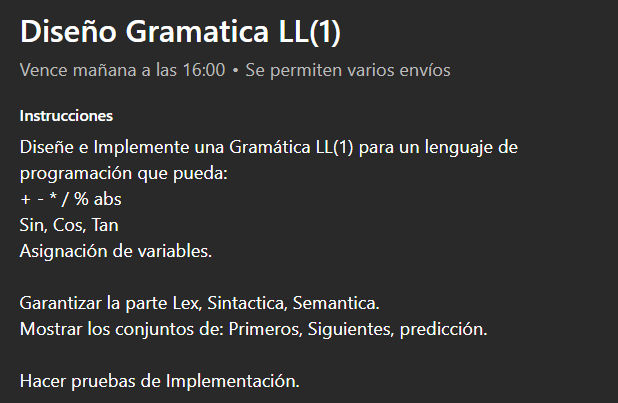
\includegraphics[width=0.72\textwidth]{enunciado.png}
\caption{Enunciado del trabajo.}
\end{figure}

Lo resolví en Python, sin librerías externas, reutilizando el programa de conjuntos del taller anterior para verificar que la gramática que diseñé sí es LL(1).

% ------------------------------------------------------------------ 2
\section{Diseño de la gramática}

\subsection{Tokens del lenguaje}

Antes de escribir las reglas definí qué va a entregar el analizador léxico. Los terminales de la gramática son clases de token, no lexemas sueltos: \tk{ID} para los nombres de variable y \tk{NUM} para los números.

\begin{table}[H]
\centering
\caption{Tokens del lenguaje.}
\small
\begin{tabular}{lll}
\toprule
Clase & Lexema & Descripción \\
\midrule
\tk{ID} & \tk{base}, \tk{x1} & nombre de variable \\
\tk{NUM} & \tk{12}, \tk{0.5} & número entero o real \\
\tk{asig} & \tk{=} & asignación \\
\tk{fin} & \tk{;} & fin de sentencia \\
\tk{mas}, \tk{menos} & \tk{+}, \tk{-} & suma y resta, y el menos unario \\
\tk{por}, \tk{entre} & \tk{*}, \tk{/} & multiplicación y división \\
\tk{modulo} & \tk{\%} & residuo entre enteros \\
\tk{abre}, \tk{cierra} & \tk{(}, \tk{)} & agrupación \\
\tk{barra} & \tk{|} & valor absoluto en forma \tk{|x|} \\
\tk{abs}, \tk{sin}, \tk{cos}, \tk{tan} & & palabras reservadas \\
\bottomrule
\end{tabular}
\end{table}

Los comentarios empiezan con \tk{\#} y llegan hasta el fin de línea; los espacios y saltos de línea se ignoran.

\subsection{Las reglas}

\noindent\begin{minipage}{\linewidth}
\begin{lstlisting}[caption={\texttt{grammars/lenguaje.txt}: la gramática del lenguaje.}]
# Gramática LL(1) del lenguaje
# Los no terminales son los símbolos de la izquierda; el resto son terminales.
# Los terminales en MAYÚSCULA son clases de token que entrega el analizador léxico.

prog     -> sents
sents    -> sent sents | ε
sent     -> ID asig expr fin

expr     -> term expr_r
expr_r   -> mas term expr_r | menos term expr_r | ε

term     -> fact term_r
term_r   -> por fact term_r | entre fact term_r | modulo fact term_r | ε

fact     -> menos fact | unidad

unidad   -> NUM
unidad   -> ID
unidad   -> abre expr cierra
unidad   -> barra expr barra
unidad   -> func abre expr cierra

func     -> abs | sin | cos | tan
\end{lstlisting}
\end{minipage}

Tomé tres decisiones para que la gramática quedara LL(1):

\begin{itemize}
  \item \textbf{Precedencia con niveles.} \nt{expr} agrupa sumas y restas, \nt{term} agrupa producto, división y módulo, y \nt{fact} es lo que va más abajo en el árbol. Como el nivel más profundo se resuelve primero, \tk{2 + 3 * 4} da 14 y no 20.
  \item \textbf{Sin recursión izquierda.} En vez de \nt{expr} $\rightarrow$ \nt{expr} \tk{+} \nt{term}, que haría que el procedimiento se llamara a sí mismo sin consumir nada, la repetición se lleva a la derecha con \nt{expr\_r} y \nt{term\_r}, que terminan en $\varepsilon$. La asociatividad por la izquierda se conserva al armar el árbol en la implementación.
  \item \textbf{Sin prefijos comunes.} Las cinco alternativas de \nt{unidad} empiezan cada una con un token distinto (\tk{NUM}, \tk{ID}, \tk{(}, \tk{|} y una función), y las cuatro funciones se agruparon en \nt{func} para que \nt{unidad} tenga una sola regla que empiece con función. Así no hay que factorizar nada.
\end{itemize}

El menos unario está en \nt{fact} $\rightarrow$ \tk{menos} \nt{fact}, que no choca con la resta binaria porque esa decisión se toma en \nt{expr\_r}, en otra posición del recorrido.

% ------------------------------------------------------------------ 3
\section{Conjuntos y verificación LL(1)}

Los conjuntos los calcula \tk{conjuntos.py}, el mismo programa del taller anterior, con algoritmos de punto fijo.

\begin{table}[H]
\centering
\caption{PRIMEROS y SIGUIENTES de la gramática.}
\footnotesize
\begin{tabular}{l p{5.0cm} p{5.4cm}}
\toprule
No terminal & PRIMEROS & SIGUIENTES \\
\midrule
\textit{prog} & \{\texttt{ID}, $\varepsilon$\} & \{\texttt{\$}\} \\
\textit{sents} & \{\texttt{ID}, $\varepsilon$\} & \{\texttt{\$}\} \\
\textit{sent} & \{\texttt{ID}\} & \{\texttt{ID}, \texttt{\$}\} \\
\textit{expr} & \{\texttt{ID}, \texttt{menos}, \texttt{NUM}, \texttt{abre}, \texttt{barra}, \texttt{abs}, \texttt{sin}, \texttt{cos}, \texttt{tan}\} & \{\texttt{fin}, \texttt{cierra}, \texttt{barra}\} \\
\textit{expr\_r} & \{\texttt{mas}, \texttt{menos}, $\varepsilon$\} & \{\texttt{fin}, \texttt{cierra}, \texttt{barra}\} \\
\textit{term} & \{\texttt{ID}, \texttt{menos}, \texttt{NUM}, \texttt{abre}, \texttt{barra}, \texttt{abs}, \texttt{sin}, \texttt{cos}, \texttt{tan}\} & \{\texttt{fin}, \texttt{mas}, \texttt{menos}, \texttt{cierra}, \texttt{barra}\} \\
\textit{term\_r} & \{\texttt{por}, \texttt{entre}, \texttt{modulo}, $\varepsilon$\} & \{\texttt{fin}, \texttt{mas}, \texttt{menos}, \texttt{cierra}, \texttt{barra}\} \\
\textit{fact} & \{\texttt{ID}, \texttt{menos}, \texttt{NUM}, \texttt{abre}, \texttt{barra}, \texttt{abs}, \texttt{sin}, \texttt{cos}, \texttt{tan}\} & \{\texttt{fin}, \texttt{mas}, \texttt{menos}, \texttt{por}, \texttt{entre}, \texttt{modulo}, \texttt{cierra}, \texttt{barra}\} \\
\textit{unidad} & \{\texttt{ID}, \texttt{NUM}, \texttt{abre}, \texttt{barra}, \texttt{abs}, \texttt{sin}, \texttt{cos}, \texttt{tan}\} & \{\texttt{fin}, \texttt{mas}, \texttt{menos}, \texttt{por}, \texttt{entre}, \texttt{modulo}, \texttt{cierra}, \texttt{barra}\} \\
\textit{func} & \{\texttt{abs}, \texttt{sin}, \texttt{cos}, \texttt{tan}\} & \{\texttt{abre}\} \\
\bottomrule
\end{tabular}
\end{table}

\begin{table}[H]
\centering
\caption{Conjuntos de PREDICCIÓN de las 24 reglas.}
\footnotesize
\begin{tabular}{r l p{6.0cm}}
\toprule
\# & Regla & PREDICCIÓN \\
\midrule
1 & \textit{prog} $\rightarrow$ \textit{sents} & \{\texttt{ID}, \texttt{\$}\} \\
2 & \textit{sents} $\rightarrow$ \textit{sent} \textit{sents} & \{\texttt{ID}\} \\
3 & \textit{sents} $\rightarrow$ $\varepsilon$ & \{\texttt{\$}\} \\
4 & \textit{sent} $\rightarrow$ \texttt{ID} \texttt{asig} \textit{expr} \texttt{fin} & \{\texttt{ID}\} \\
5 & \textit{expr} $\rightarrow$ \textit{term} \textit{expr\_r} & \{\texttt{ID}, \texttt{menos}, \texttt{NUM}, \texttt{abre}, \texttt{barra}, \texttt{abs}, \texttt{sin}, \texttt{cos}, \texttt{tan}\} \\
6 & \textit{expr\_r} $\rightarrow$ \texttt{mas} \textit{term} \textit{expr\_r} & \{\texttt{mas}\} \\
7 & \textit{expr\_r} $\rightarrow$ \texttt{menos} \textit{term} \textit{expr\_r} & \{\texttt{menos}\} \\
8 & \textit{expr\_r} $\rightarrow$ $\varepsilon$ & \{\texttt{fin}, \texttt{cierra}, \texttt{barra}\} \\
9 & \textit{term} $\rightarrow$ \textit{fact} \textit{term\_r} & \{\texttt{ID}, \texttt{menos}, \texttt{NUM}, \texttt{abre}, \texttt{barra}, \texttt{abs}, \texttt{sin}, \texttt{cos}, \texttt{tan}\} \\
10 & \textit{term\_r} $\rightarrow$ \texttt{por} \textit{fact} \textit{term\_r} & \{\texttt{por}\} \\
11 & \textit{term\_r} $\rightarrow$ \texttt{entre} \textit{fact} \textit{term\_r} & \{\texttt{entre}\} \\
12 & \textit{term\_r} $\rightarrow$ \texttt{modulo} \textit{fact} \textit{term\_r} & \{\texttt{modulo}\} \\
13 & \textit{term\_r} $\rightarrow$ $\varepsilon$ & \{\texttt{fin}, \texttt{mas}, \texttt{menos}, \texttt{cierra}, \texttt{barra}\} \\
14 & \textit{fact} $\rightarrow$ \texttt{menos} \textit{fact} & \{\texttt{menos}\} \\
15 & \textit{fact} $\rightarrow$ \textit{unidad} & \{\texttt{ID}, \texttt{NUM}, \texttt{abre}, \texttt{barra}, \texttt{abs}, \texttt{sin}, \texttt{cos}, \texttt{tan}\} \\
16 & \textit{unidad} $\rightarrow$ \texttt{NUM} & \{\texttt{NUM}\} \\
17 & \textit{unidad} $\rightarrow$ \texttt{ID} & \{\texttt{ID}\} \\
18 & \textit{unidad} $\rightarrow$ \texttt{abre} \textit{expr} \texttt{cierra} & \{\texttt{abre}\} \\
19 & \textit{unidad} $\rightarrow$ \texttt{barra} \textit{expr} \texttt{barra} & \{\texttt{barra}\} \\
20 & \textit{unidad} $\rightarrow$ \textit{func} \texttt{abre} \textit{expr} \texttt{cierra} & \{\texttt{abs}, \texttt{sin}, \texttt{cos}, \texttt{tan}\} \\
21 & \textit{func} $\rightarrow$ \texttt{abs} & \{\texttt{abs}\} \\
22 & \textit{func} $\rightarrow$ \texttt{sin} & \{\texttt{sin}\} \\
23 & \textit{func} $\rightarrow$ \texttt{cos} & \{\texttt{cos}\} \\
24 & \textit{func} $\rightarrow$ \texttt{tan} & \{\texttt{tan}\} \\
\bottomrule
\end{tabular}
\end{table}

El criterio LL(1) es que las reglas de un mismo no terminal tengan conjuntos de predicción disjuntos. El programa lo revisa par por par y confirma que se cumple:

\begin{lstlisting}
¿ES LL(1)? SÍ: las reglas de cada no terminal tienen predicciones disjuntas.
\end{lstlisting}

Se ve en la tabla anterior: las tres reglas de \nt{expr\_r} predicen \tk{mas}, \tk{menos} y el resto (\tk{fin}, \tk{cierra}, \tk{barra}), sin cruzarse; y las cinco de \nt{unidad} predicen cada una un token distinto.

% ------------------------------------------------------------------ 4
\section{Implementación}

El trabajo quedó dividido en un módulo por fase, igual que el esquema del compilador visto en clase.

\subsection{Análisis léxico}

\tk{lexico.py} recorre el texto carácter por carácter y arma la lista de tokens. Reconoce números enteros y reales, identificadores, palabras reservadas, los símbolos del lenguaje y los comentarios. Cada token guarda su línea y columna, que es lo que permite reportar los errores con la posición exacta:

\begin{lstlisting}
Error léxico: línea 2, columna 7: símbolo no reconocido '@'.
\end{lstlisting}

\subsection{Análisis sintáctico}

\tk{sintactico.py} es un analizador descendente recursivo: hay una función por cada no terminal de la gramática, y cada una decide qué regla aplicar mirando un solo token de anticipación, con los conjuntos de predicción de la tabla anterior. No hay retroceso.

Las funciones de \nt{expr\_r} y \nt{term\_r} reciben el operando izquierdo ya construido y van armando el árbol hacia la izquierda; por eso \tk{10 - 3 - 2} da 5 y no 9, aunque la gramática repita por la derecha.

El resultado es el árbol sintáctico, representado con tuplas como \tk{('bin', '*', izq, der, linea)}. Los errores también salen con posición:

\begin{lstlisting}
Error sintáctico: línea 3, columna 1: se esperaba ';' y se encontró 'y'.
\end{lstlisting}

\subsection{Análisis semántico}

\tk{semantico.py} recorre el árbol y revisa lo que la gramática no puede revisar sola. Mantiene una tabla de símbolos y aplica estas reglas:

\begin{itemize}
  \item una variable no se puede usar si no fue asignada antes;
  \item \tk{+}, \tk{-} y \tk{*} dan entero si los dos operandos son enteros, y real en cualquier otro caso;
  \item \tk{/} siempre da real;
  \item \tk{\%} solo se permite entre enteros;
  \item no se puede dividir entre la constante cero;
  \item \tk{sin}, \tk{cos} y \tk{tan} reciben radianes y devuelven real; \tk{abs} y \tk{|x|} conservan el tipo.
\end{itemize}

\begin{lstlisting}
Error semántico: línea 2: la variable 'y' se usa sin haber sido asignada.
Error semántico: línea 2: el módulo '%' solo se puede usar entre enteros (se recibió real y entero).
\end{lstlisting}

Después del análisis, una segunda pasada evalúa el programa y llena la tabla con el valor de cada variable, que es lo que se imprime al final.

% ------------------------------------------------------------------ 5
\section{Pruebas de implementación}

En \tk{test\_implementacion.py} hay 31 pruebas automáticas con \tk{unittest}, repartidas así:

\begin{table}[H]
\centering
\caption{Grupos de pruebas.}
\small
\begin{tabular}{l r p{8.0cm}}
\toprule
Grupo & Pruebas & Qué revisa \\
\midrule
Léxico & 6 & tokens, comentarios, reales, símbolos inválidos \\
Sintáctico & 9 & precedencia, asociatividad, paréntesis, menos unario, errores \\
Semántico & 6 & tipos, variable sin asignar, módulo con reales, división por cero \\
Funciones & 3 & \tk{sin}, \tk{cos}, \tk{tan} y funciones anidadas \\
Gramática & 5 & LL(1), sin recursión izquierda, PRIMEROS, SIGUIENTES y PREDICCIÓN \\
Ejemplos & 2 & los archivos de \tk{ejemplos/} dan el resultado y el error esperados \\
\bottomrule
\end{tabular}
\end{table}

Las pruebas de precedencia y asociatividad son las que muestran que la gramática quedó bien diseñada: si los niveles \nt{expr} / \nt{term} / \nt{fact} estuvieran mal, \tk{2 + 3 * 4} daría 20. Y la prueba de la gramática verifica que no hay conflictos LL(1) sobre el archivo real, no sobre una copia escrita a mano.

\begin{lstlisting}[caption={Comandos usados.}]
chmod +x run_all.sh
./run_all.sh                        # pruebas, conjuntos y ejemplos
python3 main.py ejemplos/demo.lp    # análisis completo de un programa
python3 main.py --conjuntos         # PRIMEROS, SIGUIENTES, PREDICCIÓN y LL(1)
\end{lstlisting}

% ------------------------------------------------------------------ 6
\section{Ejemplo completo}

\noindent\begin{minipage}{\linewidth}
\begin{lstlisting}[caption={\texttt{ejemplos/demo.lp}.}]
# Programa de prueba del lenguaje

base = 12;
altura = 5;
area = base * altura / 2;

resto = 17 % base;
desfase = |3 - 10|;
negativo = -base + 4;

angulo = 0.7853981634;          # 45 grados en radianes
razon = sin(angulo) / cos(angulo);
mezcla = abs(-2.5) * (base + 1) - tan(0.0);
\end{lstlisting}
\end{minipage}

\noindent\begin{minipage}{\linewidth}
\begin{lstlisting}[caption={Salida de \texttt{python3 main.py ejemplos/demo.lp}.}]
[1] Análisis léxico: 72 tokens reconocidos.
[2] Análisis sintáctico: 9 sentencias, sin errores.
[3] Análisis semántico: tipos correctos y variables asignadas antes de usarse.

Resultados
  base     = 12   (entero)
  altura   = 5   (entero)
  area     = 30.0   (real)
  resto    = 5   (entero)
  desfase  = 7   (entero)
  negativo = -8   (entero)
  angulo   = 0.785398   (real)
  razon    = 1.0   (real)
  mezcla   = 32.5   (real)
\end{lstlisting}
\end{minipage}

Se puede comprobar a mano: \tk{area} es $12 \times 5 / 2 = 30$ y queda real porque hay una división; \tk{resto} es $17 \bmod 12 = 5$ y queda entero; \tk{desfase} es $|3-10| = 7$; y \tk{razon} es $\tan(45^\circ) = 1$ calculado como seno sobre coseno.

% ------------------------------------------------------------------ 7
\section{Conclusiones}

\begin{itemize}
  \item La gramática quedó LL(1) por diseño, no por casualidad: los niveles de precedencia, la repetición por la derecha y el agrupar las funciones en un solo no terminal son las tres decisiones que evitan recursión izquierda y prefijos comunes.
  \item Los conjuntos de predicción no son solo un ejercicio de papel: son exactamente las condiciones de los \tk{if} del analizador descendente recursivo.
  \item La separación en tres módulos hace que cada error quede donde corresponde. Un símbolo raro lo detecta el léxico, un \tk{;} faltante lo detecta el sintáctico y una variable sin asignar solo se puede detectar en el semántico, porque la gramática no tiene cómo saberlo.
  \item Las 31 pruebas cubren las tres fases y la gramática, así que cualquier cambio que rompa la precedencia o introduzca un conflicto LL(1) se nota de inmediato.
\end{itemize}

\end{document}
